\newpage
\chapter{Multiplanární rekonstrukce}
Po předvedení programu v IKEM byl vznesen další požadavek na funkčnost programu a to implementace multiplanární rekonstrukce (MPR).

Multiplanární rekonstrukce je specifický způsob zobrazení snímku: Obrazovka je rozdělena na tři části. V každé části vidíme řez třírozměrného snímku a to ve třech na sebe kolmých rovinách. V každém z řezů dále vidíme vyznačené průsečíky se zbylými dvěma rovinami (viz Obrázek \ref{MPR}).

\begin{figure}
	\caption{Multiplanární rekonstrukce v programu \cite{volux}, na obrazovce je vidět snímek lidské lebky ve třech řezech (zepředu, z profilu, zespodu) a dále modelování objemu - to součástí DicomPresenteru nebude.}
	\begin{center}
	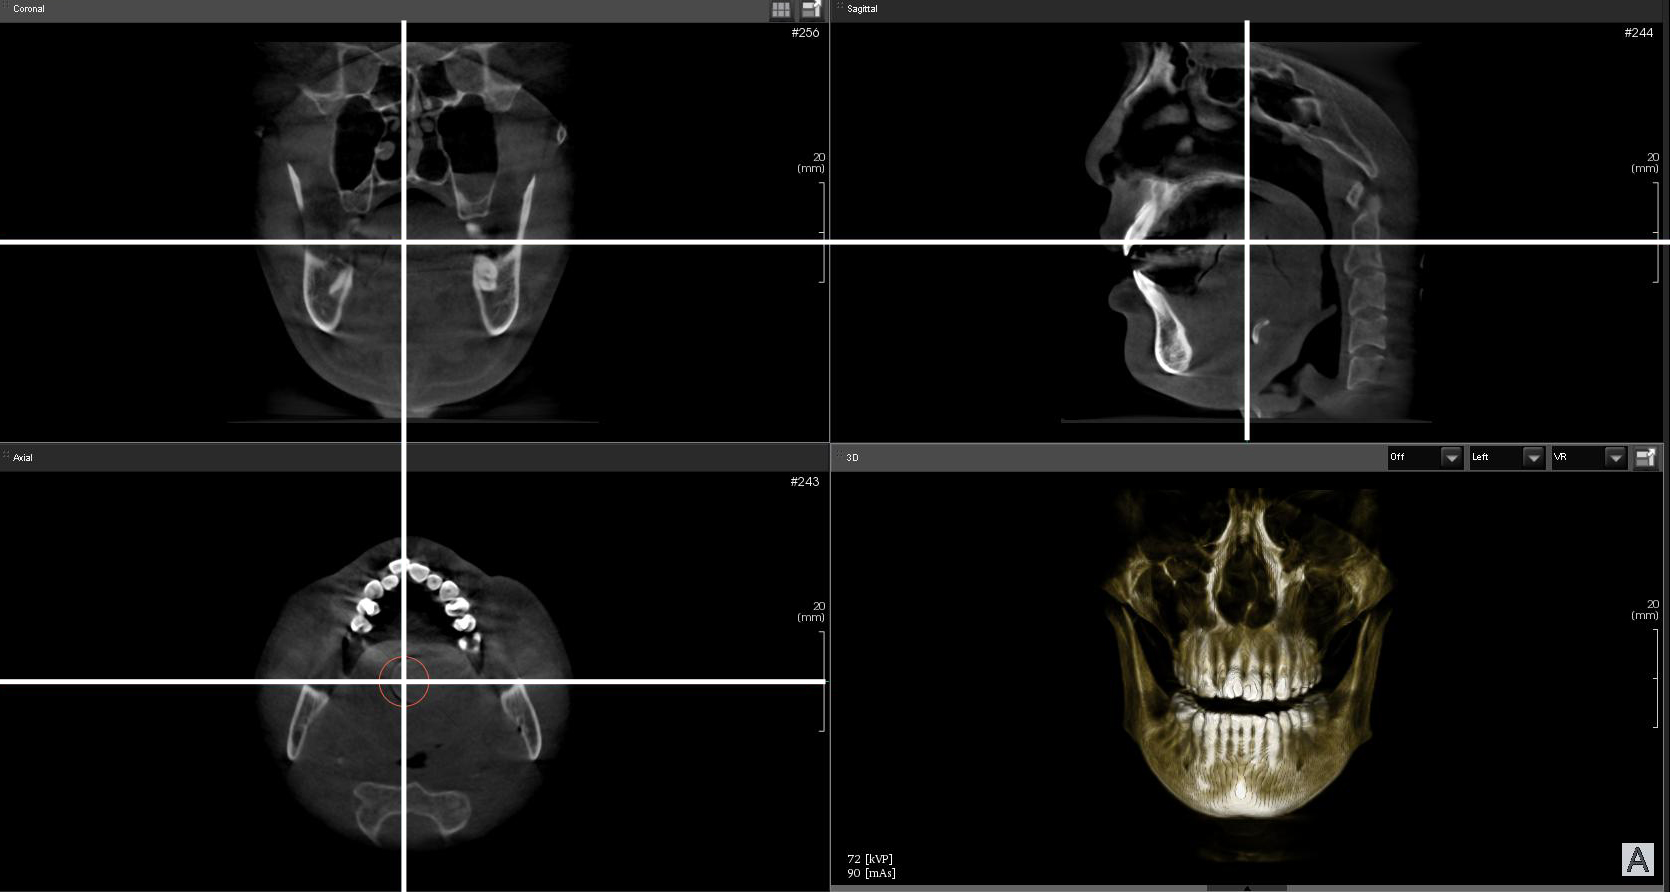
\includegraphics[width=0.7\textwidth]{Text/IMG/MPR.jpg}
	\end{center}
	\label{MPR}
\end{figure}

\section{Objektový návrh Dicom-Presenteru}
Zadání bylo do stávajícího programu přidat podporu multiplanární rekonstrukce. Jelikož přidání MPR znamená zásah do stávajícího objektového návrhu programu, je nutné se nejprve stručně seznámit se stávajícím objektovým návrhem programu.

V programu DicomPresenter je správa a vykreslování snímků řešeno použitím pěti základních tříd: Třída \clist{Image} reprezentuje snímek magnetické resonance. Třída \clist{Workspace} reprezentuje pracovní plochu na které máme otevřeno několik snímků typu \clist{Image}. Třída \clist{ImageExplorer} má na starost uložení snímků typu \clist{Image} v paměti počítače. Třídy \clist{WorkspaceExplorer} a \clist{WorkspaceManager} pak mají na starost přepínání mezi pracovními plochami a jejich uložení v paměti\footnote{Třídy \clist{Image}, \clist{Workspace}, \clist{ImageExplorer} mají na starost uložení dat v paměti i vykreslení dat na obrazovku a komunikaci s uživatelem. V případě správy pracovních ploch, kde je situace komplikovanější, jsou od sebe správa paměti a správa uživatelského rozhraní odděleny (třídy \clist{WorkspaceExplorer} a \clist{WorkspaceManager}). }. Náčrtek vztahů mezi třídami je na obrázku \ref{model}.

\begin{figure}
	\caption{Vztahy mezi objekty DicomPresenteru zajišťujícími správu pracovních ploch.}
	\begin{center}
		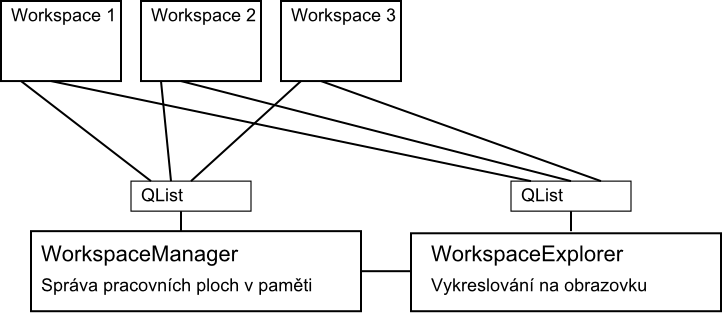
\includegraphics[width=0.7\textwidth]{Text/IMG/WorkspaceManager.png}
	\end{center}
	\label{model}
\end{figure}

Do tohoto modelu je nutné někam zařadit novou třídu, která zajistí funkčnost multiplanární rekonstrukce. Funkcemi multiplanární rekonstrukce nahrazuje to, co má na starosti třída Workspace. Otázkou bylo, zda vytvořit zcela novou třídu, nebo zda vložit nové funkce do stávající třídy Workspace, nebo zda rozdělit stávající třídu Workspace na dvě části a funkce společné pro oba typy pracovních ploch dědit. Po diskuzi byla vybrána první možnost a byla tak vytvořena třída nová, která nebude zobrazovat několik různých Dicom snímků, ale bude zobrazovat vždy jen jeden Dicom snímek v různých řezech. Bylo nutné zaručit, aby uživatel mohl přepínat mezi novou pracovní plochou s multiplanární rekonstrukcí a mezi všemi starými pracovními plochami.

\begin{comment}
\begin{figure}
	\caption{Vztahy mezi objekty DicomPresenteru zajišťujícími správu pracovních ploch.}
	\begin{center}
		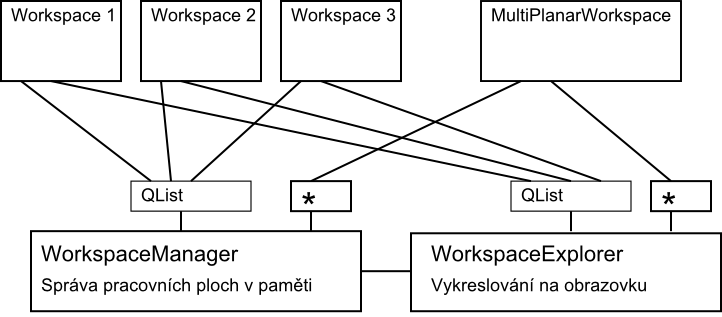
\includegraphics[width=0.7\textwidth]{Text/IMG/MultiPlanar.png}
	\end{center}
	\label{model}
\end{figure}
\end{comment}

\section{Implementace multiplanární rekonstrukce}
Multiplanární rekonstrukce byla naprogramována vytvořením nové třídy odpovídající pracovní ploše: PlanarWorkspace a dále úpravami v existující třídě Image.

\subsection{Třída PlanarWorkspace}
V třídě lze odlišit dvě části: funkce zpracovávající uživatelské akce, funkce zajišťující vykreslování výsledku na obrazovku.

Uživatelské akce jsou zachycovány funkcemi Qt knihovny \clist{QMouse\-Event\-::mouse\-Move\-Event()},\clist{QMouse\-Event\-::mouse\-Press\-Event()}. V odpovídajících funkcích z pozice kurzoru zjistíme s jakým řezem a jak má uživatel v úmyslu manipulovat\footnote{Uživatelské akce standardně zachycuje okno programu (třída Widget). Při stisku tlačítka myši třída Widget projde všechny základní prvky na obrazovce (\clist{Workspace}, \clist{WorkspaceExplorer} a \clist{WorkspaceManager}) a zjistí na který z nich uživatel klikl, všechny další akce pak směřuje tomuto prvku.}, to si uložíme do paměti počítače do proměnné \clist{planarCrossPosition}.

\begin{lstlisting}[label=DicomImageClass,caption={První část souboru \texttt{Window.cpp} se zdrojovým kódem třídy reprezentující okno programu.}]
void CGLPlanarWorkspace::mousePressEvent(QMouseEvent *event){
	if((event->x() < this->GetSize().x()/2)&&(event->y() < this->GetSize().y()/2)){
		UserManipulatingSlice = 'z';
		CGLWidget::GetInstance()->setCursor(QCursor(Qt::BlankCursor));
		iEventHistory->setX(event->x());	
		iEventHistory->setY(event->y());
		*iCursorHistory = QCursor::pos();
	}
  ...
}

void CGLPlanarWorkspace::mouseMoveEvent(QMouseEvent *event){
	QCursor::setPos(*iCursorHistory);
	if(UserManipulatingSlice == 'z'){
		int dx = event->x() - iEventHistory->x();
		int dy = iEventHistory->y() - event->y();
		if ((iPlanarCrossPosition.x+(float)dx/(float)iSensitivity>0.) && (iPlanarCrossPosition.x+(float)dx/(float)iSensitivity<1.))
			iPlanarCrossPosition.x=iPlanarCrossPosition.x+(float)dx/(float)iSensitivity;
		if ((iPlanarCrossPosition.y+(float)dy/(float)iSensitivity>0.) && (iPlanarCrossPosition.y+(float)dy/(float)iSensitivity<1.))
			iPlanarCrossPosition.y=iPlanarCrossPosition.y+(float)dy/(float)iSensitivity;
	}
	if(UserManipulatingSlice == 'x'){
 		...
	}
	if(UserManipulatingSlice == 'y'){
 		...
	}
	CGLWidget::GetInstance()->updateGL();
\end{lstlisting}

Vykreslování je řešeno ve funkci \clist{QGLWidget\-::Paint()}, to je třída Qt knihovny, kterou si předefinujeme podle potřeb. Ve funkci voláme nově definované funkce třídy \clist{Image}. Nejprve si vykreslíme tři požadované řezy do paměti grafické karty (frame buffer), pak kreslíme řezy na odpovídající místo na obrazovce. Souřadnice řezů jsou dopočítány podle proměnné \clist{planarCrossPosition}.

\begin{lstlisting}[label=DicomImageClass,caption={První část souboru \texttt{Window.cpp} se zdrojovým kódem třídy reprezentující okno programu.}]
void CGLImage::DrawToTextureSliceZ(TPlanarCrossPosition crossposition){
	glBindFramebufferEXT(GL_FRAMEBUFFER_EXT, iFBOZ);
	glBindTexture(GL_TEXTURE_3D, iTexture->GetTextureID());
	glBindTexture(GL_TEXTURE_2D, iSliceZ);
	glBegin(GL_QUADS);
	glColor4f(1.,0.,0.,1.);
	  glTexCoord3d(0,1,crossposition.z);  glVertex2d(0,0);
	  glTexCoord3d(1,1,crossposition.z);  glVertex2d(1,0);
	  glTexCoord3d(1,0,crossposition.z);  glVertex2d(1,1);
	  glTexCoord3d(0,0,crossposition.z);  glVertex2d(0,1);
	glEnd();
	glBindFramebufferEXT(GL_FRAMEBUFFER_EXT, 0);
}

void CGLImage::DrawSliceZ(){
	glBindTexture(GL_TEXTURE_2D, iSliceZ);
	glBegin(GL_QUADS);
	  glTexCoord2d(0,0);  glVertex2d(0,0.5);
	  glTexCoord2d(1,0);  glVertex2d(0.5,0.5);
	  glTexCoord2d(1,1);  glVertex2d(0.5,1);
	  glTexCoord2d(0,1);  glVertex2d(0,1);
	glEnd();
}
\end{lstlisting}





